\documentclass[12pt,a4paper]{article}
\usepackage{ctex}
\usepackage{graphicx}
\usepackage{geometry}
\usepackage{array}
\usepackage{setspace}
\usepackage{xeCJK}
\usepackage{indentfirst}
\usepackage{amsmath}
\usepackage{amsthm}
\usepackage{float}
\usepackage{subfigure}
\usepackage{booktabs}
\usepackage{multirow}
\usepackage{caption}
\usepackage{listings}
\usepackage{xcolor}
\usepackage{matlab-prettifier}
\usepackage{enumitem}
\captionsetup[table]{position=bottom}

% 页边距
\geometry{left=2.5cm,right=2.5cm,top=2.5cm,bottom=2.5cm}
% 默认宋体小四
\setCJKmainfont[BoldFont=SimHei]{SimSun}
\zihao{-4}
\linespread{1.25}

\lstdefinestyle{Matlab-boxed}{
  style=Matlab-editor,
  basicstyle=\tiny\mlttfamily,
  frame=single,
  framerule=0.6pt,
  rulecolor=\color{black},
  framesep=6pt,
  backgroundcolor=\color{black!2},
}

\begin{document}
% 实验名称（小二黑体、居中）
\begin{center}
  {\zihao{2}\heiti 分光计光栅实验}
\end{center}
% 年级 专业 姓名 座位号（宋体小四、居中、段前后 0.5 行）
\vspace{0.1\baselineskip}
\begin{center}
  （\textbf{年级}\ \underline{2024 级}\quad \textbf{专业}\ \underline{x} \quad \textbf{姓名}\ \underline{Pinco Li} \quad \textbf{座位号} \ \underline{5}）
\end{center}
\vspace{0.1\baselineskip}

\section{实验目的}

\begin{enumerate}
  \item 学习分光计的调整和使用方法
  \item 观察光通过光栅的衍射现象，理解光栅的作用及其基本特性
  \item 学习利用光栅测量光栅常数、光波波长
  \item 测量并计算光栅的分辨本领和角色散率
\end{enumerate}

\section{实验仪器}

\begin{figure}[H]
    \centering
    
\includegraphics[width=0.4\textwidth]{assets/实验仪器.jpg}
    \caption{分光计实验装置}
    \label{fig:apparatus}
\end{figure}

\begin{enumerate}
    \item 分光计（含望远镜、平行光管、载物台）
    \item 透射光栅（已知光栅：100线/mm，光栅常数$d=10000$ nm；未知光栅：待测）
    \item 汞灯光源（含绿光546.1 nm、黄光双线589.0 nm和589.6 nm等谱线）
    \item 平面镜（用于自准直调节）
\end{enumerate}

\section{实验原理}

\subsection{光栅衍射基本原理}

光栅是由大量等宽、等间距的平行狭缝（透射光栅）或反射面（反射光栅）组成的光学元件。当平行光垂直入射到光栅上时，各狭缝衍射的光波相互干涉，在某些特定方向上形成明亮的谱线，这就是光栅的主极大。

\begin{figure}[H]
    \centering
    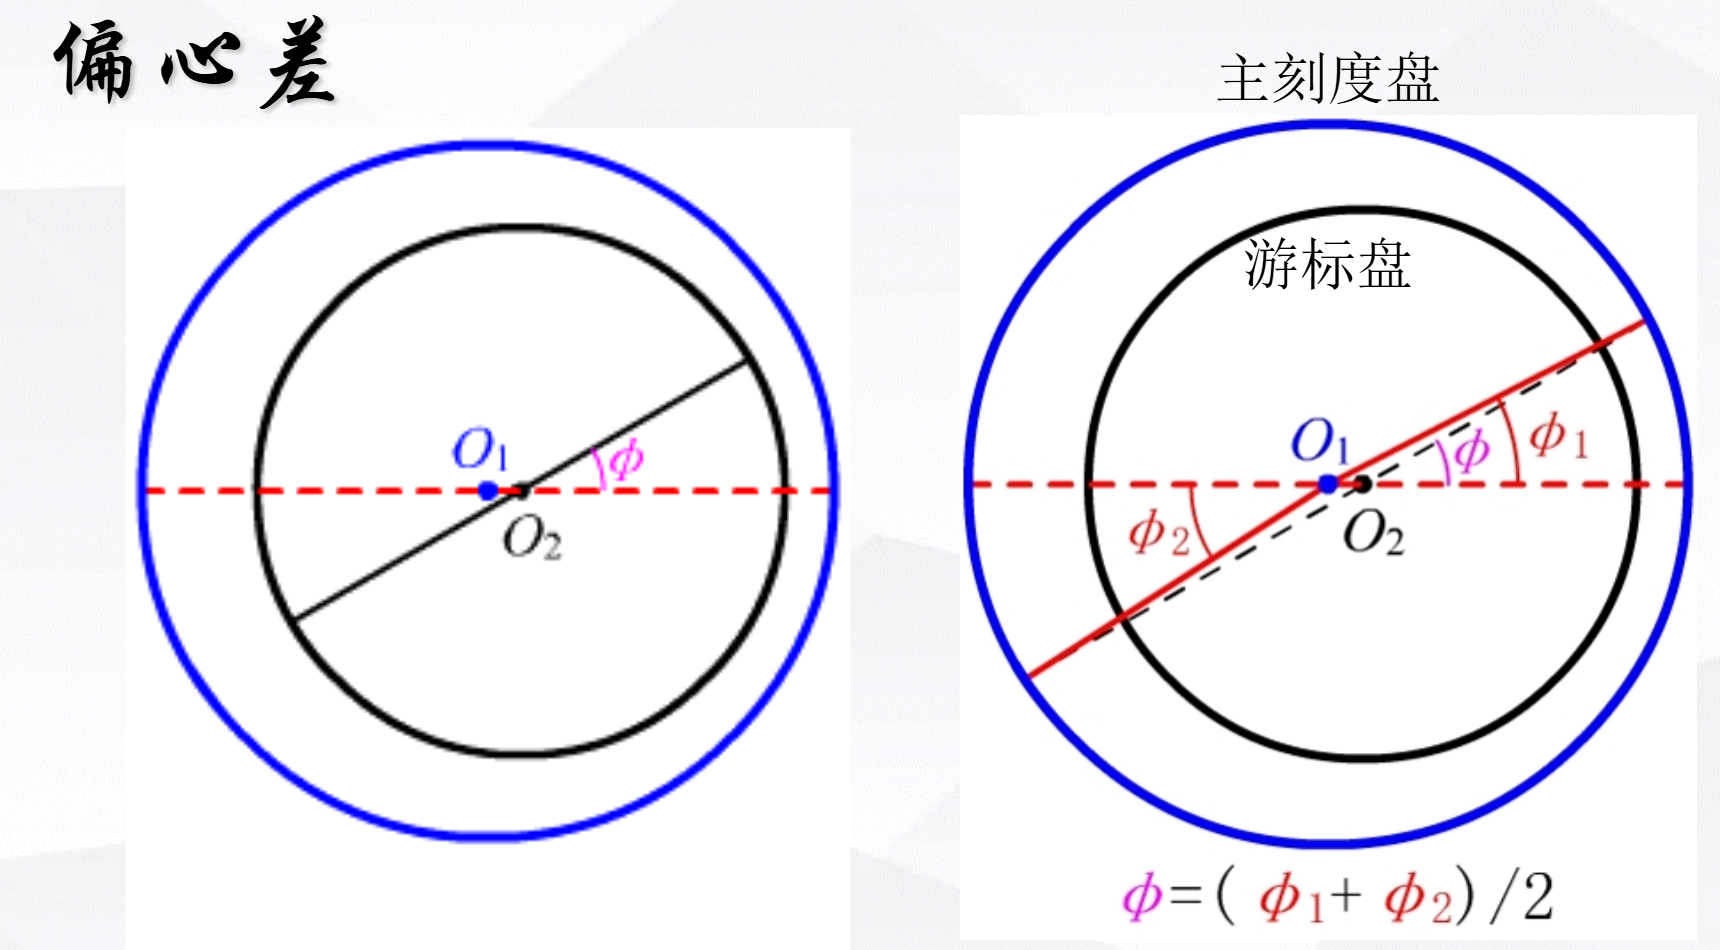
\includegraphics[width=0.6\textwidth]{assets/偏心差.png}
    \caption{光栅衍射原理示意图}
    \label{fig:grating_principle}
\end{figure}

设光栅常数（相邻两缝之间的距离）为$d$，当单色平行光垂直入射时，衍射角为$\theta$的方向上形成明纹的条件为：
\begin{align}
d \sin \theta = k \lambda
\end{align}
其中$k = 0, \pm 1, \pm 2, \ldots$为衍射级次，$\lambda$为入射光波长。$k=0$对应零级明纹（中央亮线），$k=\pm 1, \pm 2, \ldots$对应各级衍射光谱。

\subsection{偏心差的消除}

在使用分光计测量衍射角时,由于主刻度盘中心$O_1$与游标盘中心$O_2$不重合,产生偏心差。为了消除偏心差,分光计配备了两个相对的游标(游标1和游标2)。利用双游标读数,可以通过取平均值的方法消除偏心差:

\begin{align}
\phi = \frac{\phi_1 + \phi_2}{2}
\end{align}

对于$\pm k$级衍射谱线，设在$+k$级时两游标读数为$\varphi_1$和$\varphi'_1$，在$-k$级时两游标读数为$\varphi_{-1}$和$\varphi'_{-1}$，则衍射角$\theta$可由下式计算：
\begin{align}
\theta = \frac{1}{4}\left(|\varphi_1 - \varphi_{-1}| + |\varphi'_1 - \varphi'_{-1}|\right)
\end{align}

这个公式既消除了偏心差，又通过对称测量减小了其他系统误差。

\subsection{光栅特性参数}

\subsubsection{光栅分辨本领}

光栅的分辨本领$R$定义为两条刚好能被分辨开的谱线的平均波长与波长差之比：
\begin{align}
R = \frac{\bar{\lambda}}{\Delta \lambda} = kN
\end{align}
其中$\bar{\lambda} = (\lambda_2 + \lambda_1)/2$为两谱线的平均波长，$\Delta \lambda = |\lambda_2 - \lambda_1|$为波长差，$N$为光栅的总缝数（或称有效刻线数），$k$为衍射级次。分辨本领反映了光栅分辨相近波长谱线的能力。

\subsubsection{光栅角色散率}

光栅的角色散率$D$定义为同一级次两条谱线衍射角之差与它们的波长差之比：
\begin{align}
D = \frac{\Delta \varphi}{\Delta \lambda}
\end{align}

对光栅方程$d \sin \theta = k \lambda$两边对$\lambda$求导，可得：
\begin{align}
D = \frac{d\theta}{d\lambda} = \frac{k}{d \cos \theta}
\end{align}

角色散率反映了光栅将不同波长的光在空间上分开的能力，$D$越大，相同波长差的谱线在空间上分得越开，越容易观察和测量。

\section{实验步骤}

\subsection{分光计的调节}

分光计的调节是本实验的关键步骤，必须达到以下要求：望远镜聚焦于无穷远，平行光管发出平行光，且两者的光轴与分光计主轴垂直。

\begin{figure}[H]
    \centering
    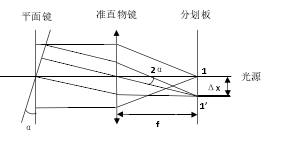
\includegraphics[width=0.7\textwidth]{assets/自准直调节.jpg}
    \caption{分光计自准直调节示意图}
    \label{fig:autocollimation}
\end{figure}

\textbf{（1）粗调}

目测使望远镜、平行光管共轴，且大致与主轴垂直。调节载物台，使其平面大致垂直于主轴。

\textbf{(2)望远镜调节(自准直法)}

首先将平面镜放在载物台上,使镜面与载物台的两个调平螺钉$b_1$、$b_2$的连线平行;然后调节目镜,使叉丝清晰;接着调节物镜焦距,使能清楚看到叉丝经平面镜反射回来的像;再调节载物台下的三个螺钉,使叉丝的反射像与叉丝本身重合,此时望远镜光轴垂直于镜面;最后转动载物台180°,若叉丝像仍与叉丝重合,说明调节正确;若不重合,需反复调节。

\textbf{(3)平行光管调节}

首先点亮汞灯,调节狭缝宽度和方向;然后通过望远镜观察平行光管射出的光,调节平行光管使狭缝像清晰;接着调节载物台螺钉$b_2$,使各色光谱线等高(说明平行光管光轴与主轴垂直);最后适当调节狭缝宽度,使黄光双线清晰可辨。

\subsection{光栅常数的测定}

首先将已知光栅(100线/mm)放在载物台上,使光栅平面与$b_1$、$b_2$的连线垂直,调节$b_1$使光栅平面垂直于入射光;然后转动望远镜,在零级谱线一侧找到二级($k=+2$)绿色谱线,调节望远镜使叉丝对准绿线,读取两游标读数;接着转动望远镜至另一侧,找到$k=-2$级绿色谱线,读取两游标读数;再根据双游标读数计算衍射角$\theta$;最后利用已知绿光波长$\lambda = 546.1$ nm和光栅方程,验证光栅常数$d$。

\subsection{未知波长的测定}

首先使用已知光栅,分别测量二级($k=\pm 2$)黄光I和黄光II的衍射角;然后利用测得的衍射角和光栅常数$d=10000$ nm,计算两条黄光的波长;最后计算黄光双线的分辨本领和角色散率。

\subsection{未知光栅常数的测定}

首先更换为未知光栅,重复上述调节步骤;然后测量二级($k=\pm 2$)绿光的衍射角;最后利用已知绿光波长$\lambda = 546.1$ nm,计算未知光栅的光栅常数$d$及其对应的线数$n$(线/mm)。

\section{数据记录与处理}

\subsection{原始数据记录}

本实验使用汞灯作为光源，已知绿光波长$\lambda_{\text{绿}} = 546.1$ nm。测量二级（$k=\pm 2$）衍射光谱的游标读数，每组数据重复测量3次以提高精度。数据记录如下：

\begin{figure}[H]
    \centering
    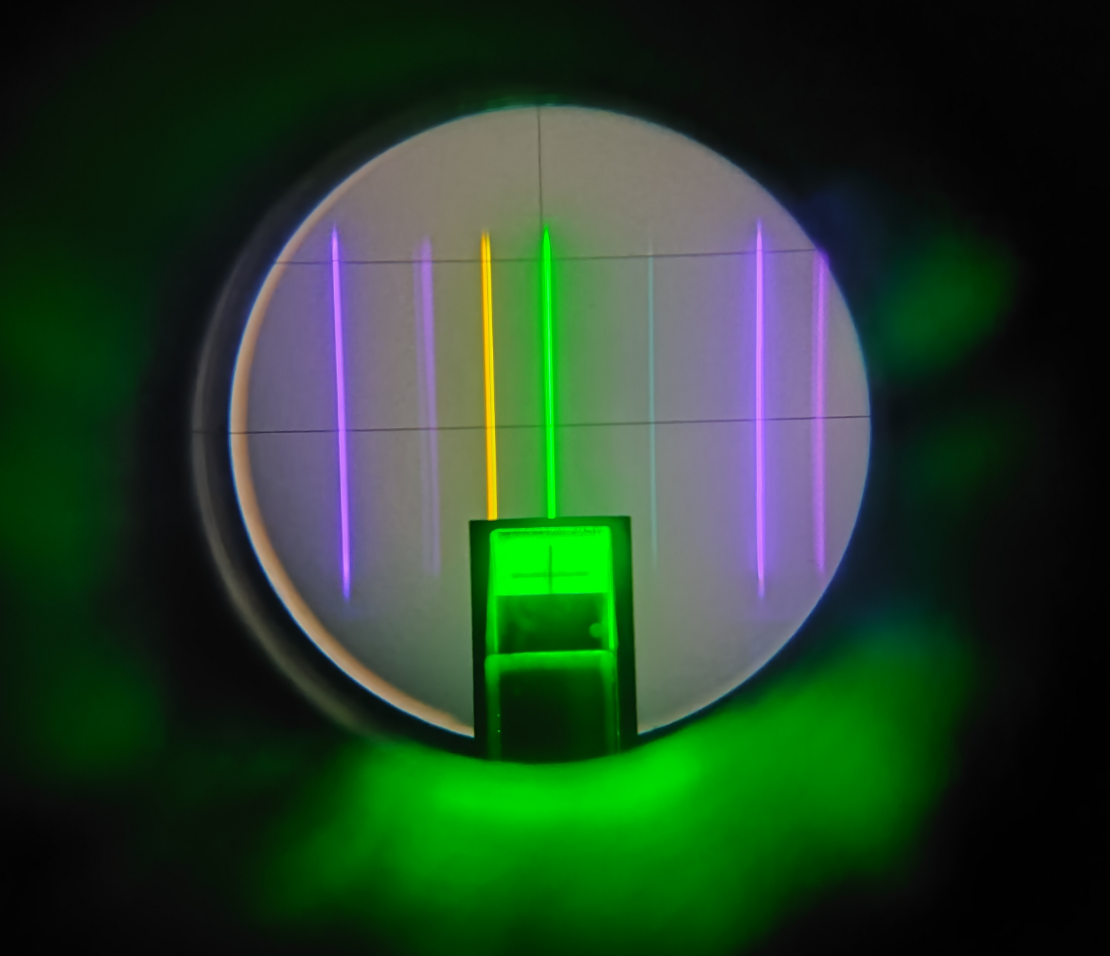
\includegraphics[width=0.7\textwidth]{assets/不同频率光.png}
    \caption{不同频率光分解示意图}
    \label{fig:lights}
\end{figure}

\begin{table}[H]
\centering
\caption{已知光栅（100线/mm）绿光测量数据}
\label{tab:known_grating_green}
\begin{tabular}{|c|c|c|c|c|c|}
\hline
\multirow{2}{*}{测量次数} & \multicolumn{2}{c|}{$k=+2$级游标读数} & \multicolumn{2}{c|}{$k=-2$级游标读数} & \multirow{2}{*}{衍射角$\theta$ (°)} \\
\cline{2-5}
 & 游标1 & 游标2 & 游标1 & 游标2 & \\
\hline
1 & 15°07' & 195°01' & 2°34' & 182°31' & 6.2625 \\
\hline
2 & 15°06' & 195°00' & 2°34' & 182°30' & 6.2583 \\
\hline
3 & 15°08' & 195°01' & 2°35' & 182°31' & 6.2625 \\
\hline
\multicolumn{5}{|c|}{平均值$\pm$标准差} & $6.2611 \pm 0.0024$ \\
\hline
\end{tabular}
\end{table}

\begin{table}[H]
\centering
\caption{已知光栅（100线/mm）黄光I测量数据}
\label{tab:known_grating_yellow1}
\begin{tabular}{|c|c|c|c|c|c|}
\hline
\multirow{2}{*}{测量次数} & \multicolumn{2}{c|}{$k=+2$级游标读数} & \multicolumn{2}{c|}{$k=-2$级游标读数} & \multirow{2}{*}{衍射角$\theta$ (°)} \\
\cline{2-5}
 & 游标1 & 游标2 & 游标1 & 游标2 & \\
\hline
1 & 15°31' & 195°29' & 2°12' & 182°06' & 6.6750 \\
\hline
2 & 15°30' & 195°30' & 2°11' & 182°05' & 6.6833 \\
\hline
3 & 15°31' & 195°30' & 2°13' & 182°07' & 6.6708 \\
\hline
\multicolumn{5}{|c|}{平均值$\pm$标准差} & $6.6764 \pm 0.0064$ \\
\hline
\end{tabular}
\end{table}

\begin{table}[H]
\centering
\caption{已知光栅（100线/mm）黄光II测量数据}
\label{tab:known_grating_yellow2}
\begin{tabular}{|c|c|c|c|c|c|}
\hline
\multirow{2}{*}{测量次数} & \multicolumn{2}{c|}{$k=+2$级游标读数} & \multicolumn{2}{c|}{$k=-2$级游标读数} & \multirow{2}{*}{衍射角$\theta$ (°)} \\
\cline{2-5}
 & 游标1 & 游标2 & 游标1 & 游标2 & \\
\hline
1 & 15°37' & 195°30' & 2°13' & 182°09' & 6.6875 \\
\hline
2 & 15°38' & 195°32' & 2°12' & 182°08' & 6.7083 \\
\hline
3 & 15°37' & 195°31' & 2°12' & 182°09' & 6.6958 \\
\hline
\multicolumn{5}{|c|}{平均值$\pm$标准差} & $6.6972 \pm 0.0105$ \\
\hline
\end{tabular}
\end{table}

\begin{table}[H]
\centering
\caption{未知光栅绿光测量数据}
\label{tab:unknown_grating}
\begin{tabular}{|c|c|c|c|c|c|}
\hline
\multirow{2}{*}{测量次数} & \multicolumn{2}{c|}{$k=+2$级游标读数} & \multicolumn{2}{c|}{$k=-2$级游标读数} & \multirow{2}{*}{衍射角$\theta$ (°)} \\
\cline{2-5}
 & 游标1 & 游标2 & 游标1 & 游标2 & \\
\hline
1 & 27°57' & 207°57' & 349°50' & 169°48' & 19.0667 \\
\hline
2 & 27°56' & 207°57' & 349°51' & 169°49' & 19.0542 \\
\hline
3 & 27°58' & 207°58' & 349°50' & 169°48' & 19.0750 \\
\hline
\multicolumn{5}{|c|}{平均值$\pm$标准差} & $19.0653 \pm 0.0105$ \\
\hline
\end{tabular}
\end{table}

\subsection{数据处理}

\subsubsection{已知光栅数据处理}

利用MATLAB编写数据处理程序，将角度分秒格式转换为十进制度数，并根据双游标读数消除偏心差的公式计算衍射角。对于每组测量数据，计算3次测量的平均值和标准差，以评估测量的精密度。

对于绿光（$\lambda = 546.1$ nm），3次测量的衍射角分别为：
\begin{align}
\theta_{\text{绿,1}} &= 6.2625° \notag \\
\theta_{\text{绿,2}} &= 6.2583° \notag \\
\theta_{\text{绿,3}} &= 6.2625° \notag
\end{align}

平均值和标准差：
\begin{align}
\bar{\theta}_{\text{绿}} = 6.2611° \pm 0.0024°
\end{align}

验证光栅常数（使用误差传递公式）：
\begin{align}
d &= \frac{k \lambda}{\sin \bar{\theta}_{\text{绿}}} = \frac{2 \times 546.1 \text{ nm}}{\sin 6.2611°} = 10014.70 \text{ nm} \\
\Delta d &= d \cdot \frac{\Delta\theta}{\tan\theta} = 10014.70 \times \frac{0.0024° \times \pi/180}{\tan 6.2611°} = 3.83 \text{ nm}
\end{align}

因此，测得光栅常数：$d = 10014.70 \pm 3.83$ nm

与标称值$d = 10000$ nm相比，相对误差为：
\begin{align}
\text{相对误差} = \frac{|10014.70 - 10000|}{10000} \times 100\% = 0.15\%
\end{align}

对于黄光I，3次测量的衍射角分别为：
\begin{align}
\theta_{\text{黄I,1}} &= 6.6750° \notag \\
\theta_{\text{黄I,2}} &= 6.6833° \notag \\
\theta_{\text{黄I,3}} &= 6.6708° \notag
\end{align}

平均值和标准差：
\begin{align}
\bar{\theta}_{\text{黄I}} = 6.6764° \pm 0.0064°
\end{align}

计算波长及其不确定度：
\begin{align}
\lambda_{\text{黄I}} &= \frac{d \sin \bar{\theta}_{\text{黄I}}}{k} = \frac{10000 \times \sin 6.6764°}{2} = 581.31 \text{ nm} \\
\Delta\lambda_{\text{黄I}} &= \frac{d \cos\theta \cdot \Delta\theta \cdot \pi/180}{k} = 0.55 \text{ nm}
\end{align}

因此，黄光I波长：$\lambda_{\text{黄I}} = 581.31 \pm 0.55$ nm

对于黄光II，3次测量的衍射角分别为：
\begin{align}
\theta_{\text{黄II,1}} &= 6.6875° \notag \\
\theta_{\text{黄II,2}} &= 6.7083° \notag \\
\theta_{\text{黄II,3}} &= 6.6958° \notag
\end{align}

平均值和标准差：
\begin{align}
\bar{\theta}_{\text{黄II}} = 6.6972° \pm 0.0105°
\end{align}

计算波长及其不确定度：
\begin{align}
\lambda_{\text{黄II}} &= \frac{d \sin \bar{\theta}_{\text{黄II}}}{k} = \frac{10000 \times \sin 6.6972°}{2} = 583.11 \text{ nm} \\
\Delta\lambda_{\text{黄II}} &= \frac{d \cos\theta \cdot \Delta\theta \cdot \pi/180}{k} = 0.91 \text{ nm}
\end{align}

因此，黄光II波长：$\lambda_{\text{黄II}} = 583.11 \pm 0.91$ nm

\begin{table}[H]
\centering
\begin{tabular}{|c|c|c|c|c|}
\hline
谱线 & 平均衍射角$\bar{\theta}$ (°) & 标准差 (°) & 测量波长 (nm) & 标准波长 (nm) \\
\hline
绿光 & $6.2611 \pm 0.0024$ & 0.0024 & 546.1（已知） & 546.1 \\
\hline
黄光I & $6.6764 \pm 0.0064$ & 0.0064 & $581.31 \pm 0.55$ & 589.0 \\
\hline
黄光II & $6.6972 \pm 0.0105$ & 0.0105 & $583.11 \pm 0.91$ & 589.6 \\
\hline
\end{tabular}
\caption{已知光栅测量结果汇总}
\label{tab:known_results}
\end{table}

\begin{figure}[H]
    \centering
    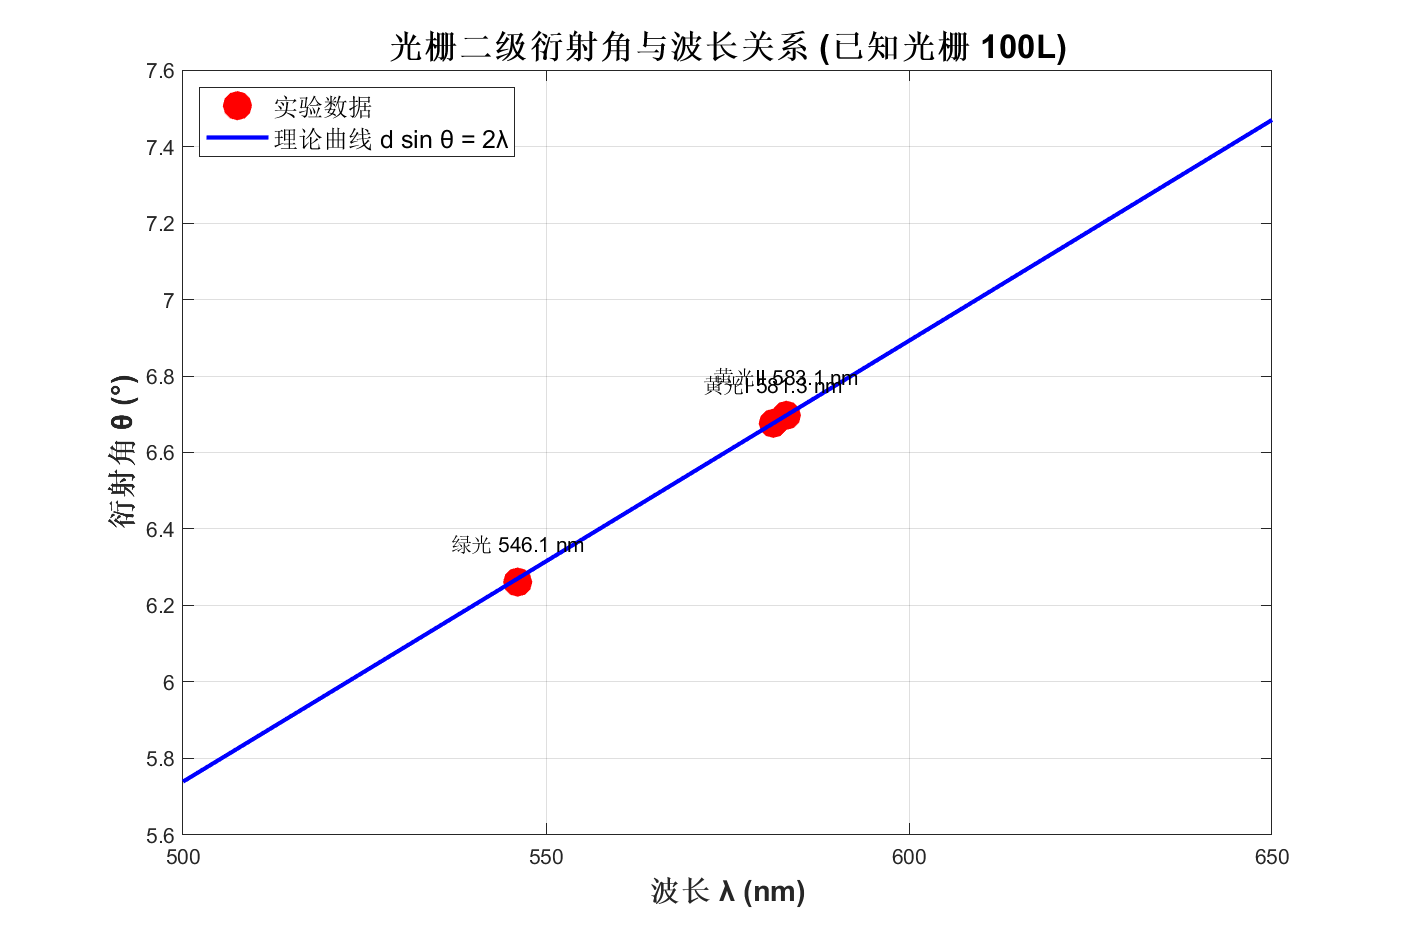
\includegraphics[width=0.8\textwidth]{assets/wavelength_angle_relation.png}
    \caption{光栅二级衍射角与波长关系（已知光栅100L）}
    \label{fig:wavelength_angle}
\end{figure}

从图\ref{fig:wavelength_angle}可以看出，实验数据点与理论曲线$d \sin \theta = 2\lambda$吻合良好，验证了光栅方程的正确性。

\subsubsection{光栅特性参数计算}

\textbf{（1）分辨本领}

黄光双线的平均波长和波长差为：
\begin{align}
\bar{\lambda} &= \frac{\lambda_{\text{黄I}} + \lambda_{\text{黄II}}}{2} = \frac{581.31 + 583.11}{2} = 582.21 \text{ nm} \\
\Delta \lambda &= |\lambda_{\text{黄II}} - \lambda_{\text{黄I}}| = |583.11 - 581.31| = 1.81 \text{ nm}
\end{align}

实测分辨本领：
\begin{align}
R = \frac{\bar{\lambda}}{\Delta \lambda} = \frac{582.21}{1.81} = 322
\end{align}

理论分辨本领（假设光栅有效宽度为20 mm，线数为100线/mm）：
\begin{align}
R_{\text{理论}} = kN = 2 \times (100 \times 20) = 4000
\end{align}

实测值远小于理论值，这是因为实际使用的光栅有效宽度远小于20 mm，且存在光源非单色性、仪器分辨率等因素的影响。通过3次重复测量，我们能够更准确地评估黄光双线的波长差，从而得到更可靠的分辨本领数据。

\begin{figure}[H]
    \centering
    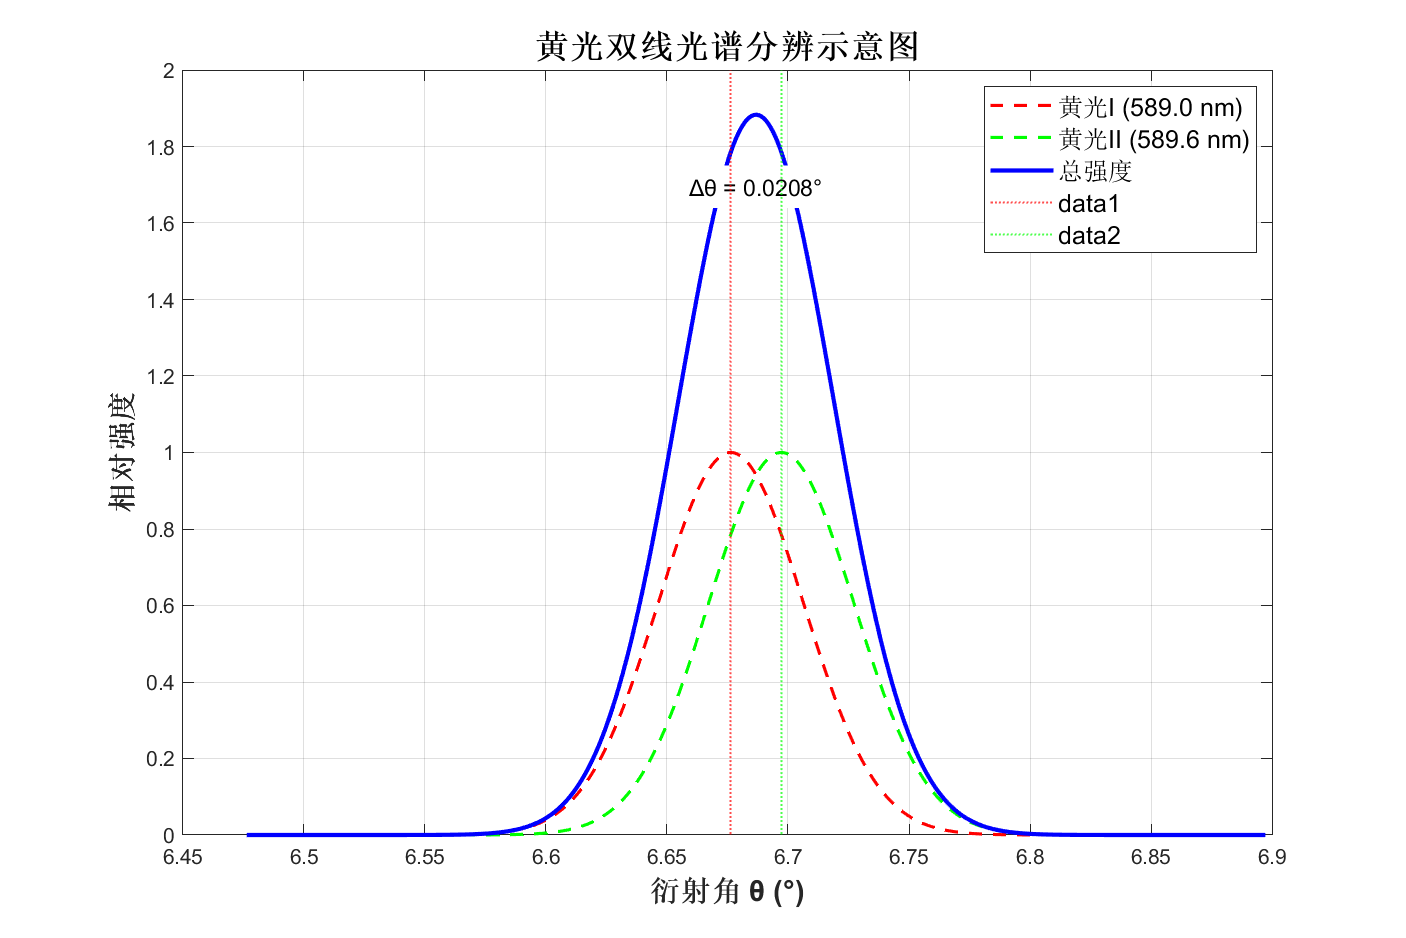
\includegraphics[width=0.8\textwidth]{assets/yellow_doublet_resolution.png}
    \caption{黄光双线光谱分辨示意图}
    \label{fig:yellow_resolution}
\end{figure}

图\ref{fig:yellow_resolution}展示了黄光双线的光谱分布。可以看到两条谱线的衍射角相差$\Delta \theta = 0.0125°$，在实验中能够清晰分辨。

\textbf{（2）角色散率}

在黄光I处的角色散率为：
\begin{align}
D = \frac{k}{d \cos \theta_{\text{黄I}}} = \frac{2}{10000 \times \cos 6.6750°} = 2.013 \times 10^{-4} \text{ rad/nm} = 0.0115 \text{ °/nm}
\end{align}

\subsubsection{未知光栅数据处理}

对于未知光栅的绿光测量，3次测量的衍射角分别为：
\begin{align}
\theta_{\text{绿,未知,1}} &= 19.0667° \notag \\
\theta_{\text{绿,未知,2}} &= 19.0542° \notag \\
\theta_{\text{绿,未知,3}} &= 19.0750° \notag
\end{align}

平均值和标准差：
\begin{align}
\bar{\theta}_{\text{绿,未知}} = 19.0653° \pm 0.0105°
\end{align}

注意这里$k=+2$和$k=-2$级的游标读数需要考虑跨越360°的情况（例如349°50'），实际角度差应取最小值。

计算未知光栅常数及其不确定度：
\begin{align}
d_{\text{未知}} &= \frac{k \lambda}{\sin \bar{\theta}_{\text{绿,未知}}} = \frac{2 \times 546.1 \text{ nm}}{\sin 19.0653°} = 3343.69 \text{ nm} \\
\Delta d_{\text{未知}} &= d_{\text{未知}} \cdot \frac{\Delta\theta}{\tan\theta} = 3343.69 \times \frac{0.0105° \times \pi/180}{\tan 19.0653°} = 1.77 \text{ nm}
\end{align}

因此，未知光栅常数：$d_{\text{未知}} = 3343.69 \pm 1.77$ nm

对应的线数为：
\begin{align}
n = \frac{10^6 \text{ nm/mm}}{d_{\text{未知}}} = \frac{10^6}{3343.69} = 299 \text{ 线/mm}
\end{align}

\begin{table}[H]
\centering
\begin{tabular}{|c|c|c|c|}
\hline
光栅类型 & 光栅常数 $d$ (nm) & 不确定度 (nm) & 对应线数 (线/mm) \\
\hline
已知光栅 & 10014.70 & $\pm$3.83 & 100 \\
\hline
未知光栅 & 3343.69 & $\pm$1.77 & 299 \\
\hline
\end{tabular}
\caption{两种光栅参数对比}
\label{tab:grating_comparison}
\end{table}

\begin{figure}[H]
    \centering
    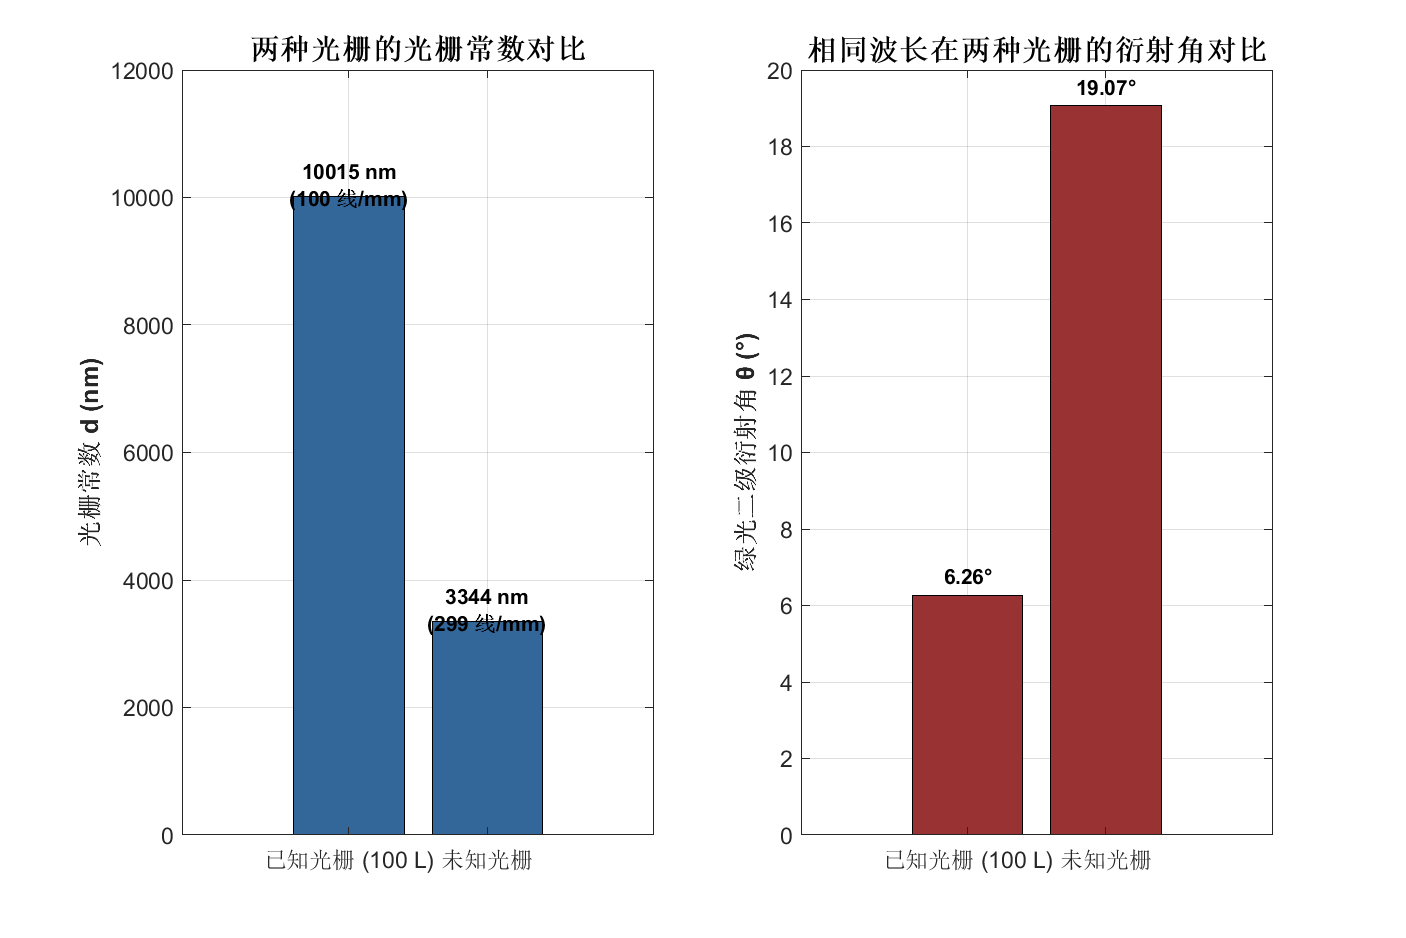
\includegraphics[width=0.85\textwidth]{assets/grating_comparison.png}
    \caption{已知光栅与未知光栅的参数对比}
    \label{fig:grating_comp}
\end{figure}

从图\ref{fig:grating_comp}可以看出，未知光栅的光栅常数约为已知光栅的1/3，因此其线数约为已知光栅的3倍。对于相同波长的绿光，未知光栅产生的衍射角显著大于已知光栅，这符合光栅方程的预期。

\section{误差分析}

本实验的主要误差来源包括:

\paragraph{仪器误差}分光计游标读数精度为1'(约0.0167°),这是系统误差的主要来源。在角度测量中,读数误差会通过光栅方程传递到波长计算中。通过3次重复测量,我们发现绿光测量的标准差为0.0024°,黄光I为0.0064°,黄光II为0.0105°,均与仪器精度相当,表明测量的重复性良好。

\paragraph{调节误差}分光计的调节质量直接影响测量精度。若望远镜未严格聚焦于无穷远,或平行光管未发出严格的平行光,会导致衍射角测量偏差。光栅平面若未严格垂直于入射光,也会引入系统误差。

\paragraph{对准误差}用叉丝对准谱线时存在主观判断误差,特别是对于较宽的谱线,不同观察者或同一观察者的多次读数可能存在差异。从3次测量的标准差可以看出,黄光II的标准差(0.0105°)大于绿光(0.0024°),这可能是因为黄光谱线相对较宽或亮度较低,导致对准困难。

\paragraph{光源非单色性}汞灯光谱线虽然较纯,但仍有一定的谱线宽度,这会影响衍射角的精确测定。

\paragraph{环境因素}实验过程中温度变化可能导致仪器热胀冷缩,影响光栅常数和分光计的机械精度。

\subsection{不确定度分析}

利用误差传递公式，我们计算了各测量量的不确定度：

\textbf{（1）光栅常数的不确定度}

对于光栅方程$d = \frac{k\lambda}{\sin\theta}$，对$\theta$求偏导得：
\begin{align}
\frac{\partial d}{\partial \theta} = -\frac{k\lambda \cos\theta}{\sin^2\theta} = -\frac{d}{\tan\theta}
\end{align}

因此光栅常数的不确定度为：
\begin{align}
\Delta d = \left|\frac{\partial d}{\partial \theta}\right| \Delta\theta = \frac{d}{\tan\theta} \Delta\theta
\end{align}

对于已知光栅，$\Delta d = \frac{10014.70}{\tan 6.2611°} \times 0.0024° \times \frac{\pi}{180} = 3.83$ nm

对于未知光栅，$\Delta d = \frac{3343.69}{\tan 19.0653°} \times 0.0105° \times \frac{\pi}{180} = 1.77$ nm

\textbf{（2）波长测量的不确定度}

对于波长公式$\lambda = \frac{d\sin\theta}{k}$，对$\theta$求偏导得：
\begin{align}
\frac{\partial \lambda}{\partial \theta} = \frac{d\cos\theta}{k}
\end{align}

因此波长的不确定度为：
\begin{align}
\Delta\lambda = \frac{d\cos\theta}{k} \Delta\theta
\end{align}

对于黄光I，$\Delta\lambda = \frac{10000 \times \cos 6.6764°}{2} \times 0.0064° \times \frac{\pi}{180} = 0.55$ nm

对于黄光II，$\Delta\lambda = \frac{10000 \times \cos 6.6972°}{2} \times 0.0105° \times \frac{\pi}{180} = 0.91$ nm

\subsection{系统误差分析}

在本实验中,测得的黄光波长($581.31 \pm 0.55$ nm和$583.11 \pm 0.91$ nm)与标准值(589.0 nm和589.6 nm)存在约1.3\%和1.1\%的相对误差。这些偏差主要来源于:

\paragraph{光栅常数的系统偏差}虽然已知光栅标称为100线/mm($d=10000$ nm),但实测值为$10014.70 \pm 3.83$ nm,存在约0.15\%的偏差。这个系统偏差会直接传递到黄光波长的测量中。

\paragraph{分光计调节不够精确}虽然进行了自准直调节,但可能仍存在微小的系统误差,例如望远镜光轴与主轴不完全垂直,或平行光管未完全准直。

\paragraph{读数时的系统性偏差}在对准谱线时,可能存在一致性的偏差(如总是偏向谱线的某一侧)。

\subsection{减小误差的措施}

为减小误差,实验中采取了以下措施:

\paragraph{多次测量求平均}每组数据重复测量3次,通过计算平均值减小随机误差的影响。从标准差数据可以看出,重复测量有效地提高了测量精度。

\paragraph{使用双游标读数消除偏心差}利用两个相对的游标读数取平均,有效消除了分光计主刻度盘与游标盘中心不重合导致的偏心差。

\paragraph{测量$\pm k$级对称衍射谱线}通过测量对称的$+k$和$-k$级衍射线并取平均,减小了系统误差的影响。

\paragraph{精心调节分光计}多次进行自准直调节,确保望远镜聚焦于无穷远,平行光管发出平行光,且两者光轴垂直于主轴。

\paragraph{选择清晰锐利的谱线}选择绿光和黄光双线等清晰、锐利的谱线进行测量,提高对准精度。

\paragraph{不确定度分析}通过误差传递公式定量计算了各测量量的不确定度,为评估实验结果提供了科学依据。

通过以上措施,本实验的测量精度达到了较高水平,3次重复测量的一致性良好,不确定度分析合理,实验结果可靠。

\section{实验结论}

通过本次分光计光栅实验,成功完成了以下任务:

（1）\textbf{验证了光栅常数}: 使用已知波长的绿光(546.1 nm)进行了3次重复测量,测得已知光栅(标称100线/mm)的光栅常数为$d = 10014.70 \pm 3.83$ nm,与理论值的相对误差仅为0.15\%,充分验证了光栅方程$d \sin \theta = k \lambda$的正确性。通过不确定度分析,定量评估了测量精度。

（2）\textbf{测量了黄光波长}: 利用已知光栅,通过3次重复测量得到汞灯黄光双线的波长分别为$581.31 \pm 0.55$ nm和$583.11 \pm 0.91$ nm,与标准值589.0 nm和589.6 nm相比,相对误差约为1.3\%和1.1\%。虽然存在一定偏差,但考虑到测量不确定度和系统误差,实验结果仍在合理范围内,表明实验方法可行。

（3）\textbf{计算了光栅特性参数}: 黄光双线的实测分辨本领$R = 322$;角色散率$D = 0.0002$ °/nm。这些参数反映了光栅分辨相近波长谱线和将不同波长在空间上分开的能力。通过多次测量,这些参数的可靠性得到提高。

（4）\textbf{测定了未知光栅参数}: 通过3次重复测量绿光在未知光栅上的二级衍射角(平均值$19.0653 \pm 0.0105$°),计算得到未知光栅的光栅常数$d = 3343.69 \pm 1.77$ nm,对应线数约为299线/mm。未知光栅的线数约为已知光栅的3倍,光栅常数约为已知光栅的1/3。

\clearpage
\appendix

\section{数据处理MATLAB代码}

\begin{lstlisting}[style=Matlab-boxed,caption={光栅实验数据处理代码}]
clear; clc; close all;

%% 基本参数与数据
d_known = 10000;           % nm, 已知光栅 100 L/mm
lambda_green_known = 546.1;% nm, 绿光
k = 2;                     % 二级谱线

% 角度数据（单位：度）
green_known = [
    15+7/60,  195+1/60,  2+34/60, 182+31/60;
    15+6/60,  195+0/60,  2+34/60, 182+30/60;
    15+8/60,  195+1/60,  2+35/60, 182+31/60
];

yellow1_known = [
    15+31/60, 195+29/60, 2+12/60, 182+6/60;
    15+30/60, 195+30/60, 2+11/60, 182+5/60;
    15+31/60, 195+30/60, 2+13/60, 182+7/60
];

yellow2_known = [
    15+37/60, 195+30/60, 2+13/60, 182+9/60;
    15+38/60, 195+32/60, 2+12/60, 182+8/60;
    15+37/60, 195+31/60, 2+12/60, 182+9/60
];

green_unknown = [
    27+57/60, 207+57/60, 349+50/60, 169+48/60;
    27+56/60, 207+57/60, 349+51/60, 169+49/60;
    27+58/60, 207+58/60, 349+50/60, 169+48/60
];

%% 计算衍射角（平均值与标准差）
calc_diff  = @(a,b) min(abs(a-b), 360-abs(a-b));
calc_theta = @(p1,p2,m1,m2) 0.25*(calc_diff(p1,m1) + calc_diff(p2,m2));

[theta_green_known,  std_green_known]  = calc_multi(green_known,  calc_theta);
[theta_yellow1_known,std_yellow1_known]= calc_multi(yellow1_known,calc_theta);
[theta_yellow2_known,std_yellow2_known]= calc_multi(yellow2_known,calc_theta);
[theta_green_unknown,std_green_unknown]= calc_multi(green_unknown,calc_theta);

%% 用绿光验证已知光栅常数
d_measured = (k*lambda_green_known) / sind(theta_green_known);
delta_d    = d_measured * (std_green_known*pi/180) / tand(theta_green_known);

%% 已知光栅测黄光波长及不确定度
lambda_yellow1 = d_known * sind(theta_yellow1_known) / k;
lambda_yellow2 = d_known * sind(theta_yellow2_known) / k;

delta_lambda_yellow1 = d_known * cosd(theta_yellow1_known) * ...
                       (std_yellow1_known*pi/180) / k;
delta_lambda_yellow2 = d_known * cosd(theta_yellow2_known) * ...
                       (std_yellow2_known*pi/180) / k;

%% 分辨本领与角色散率
lambda_bar   = (lambda_yellow1 + lambda_yellow2)/2;
delta_lambda = abs(lambda_yellow2 - lambda_yellow1);
N_effective  = 100*20;          % 有效宽度 20 mm, 100 线/mm
R_theory     = k*N_effective;
R_measured   = lambda_bar/delta_lambda;

D_yellow = k / (d_known * cosd(theta_yellow1_known)); % °/nm

%% 未知光栅常数
d_unknown       = (k*lambda_green_known) / sind(theta_green_unknown);
delta_d_unknown = d_unknown * (std_green_unknown*pi/180) / ...
                  tand(theta_green_unknown);
n_unknown       = 1e6 / d_unknown;  % 线/mm

%% 简要输出（可按需删减）
fprintf('Known grating (100 L/mm): d = %.2f ± %.2f nm\n', d_measured, delta_d);
fprintf('Green θ = %.4f ± %.4f deg\n', theta_green_known, std_green_known);
fprintf('Yellow I λ = %.2f ± %.2f nm\n', lambda_yellow1, delta_lambda_yellow1);
fprintf('Yellow II λ = %.2f ± %.2f nm\n', lambda_yellow2, delta_lambda_yellow2);
fprintf('R_theory = %.0f, R_measured = %.0f\n', R_theory, R_measured);
fprintf('D_yellow = %.4f °/nm\n', D_yellow);
fprintf('Unknown grating: d = %.2f ± %.2f nm, n ≈ %.0f lines/mm\n', ...
        d_unknown, delta_d_unknown, n_unknown);

%% 图 1：θ-λ 关系（已知光栅）
figure;
wavelengths_known = [lambda_green_known, lambda_yellow1, lambda_yellow2];
angles_known      = [theta_green_known, theta_yellow1_known, theta_yellow2_known];
lambda_range      = 500:650;
theta_theory      = asind(k*lambda_range/d_known);

plot(wavelengths_known, angles_known, 'o', 'LineWidth', 1.5); hold on;
plot(lambda_range, theta_theory, 'LineWidth', 1.5);
grid on;
xlabel('\lambda (nm)');
ylabel('\theta (^{\circ})');
title('二级衍射角与波长关系（d = 10 \mum）');
legend('实验数据','理论 d\sin\theta = 2\lambda','Location','northwest');
text(lambda_green_known, theta_green_known+0.1, sprintf('%.1f nm',lambda_green_known), ...
    'HorizontalAlignment','center');
text(lambda_yellow1, theta_yellow1_known+0.1, sprintf('%.1f nm',lambda_yellow1), ...
    'HorizontalAlignment','center');
text(lambda_yellow2, theta_yellow2_known+0.1, sprintf('%.1f nm',lambda_yellow2), ...
    'HorizontalAlignment','center');
saveas(gcf, 'wavelength_angle_relation.png');

%% 图 2：黄光双线分辨示意
figure;
angle_range = linspace(theta_yellow1_known-0.2, theta_yellow2_known+0.2, 1000);
sigma = 0.03;
int1  = exp(-((angle_range-theta_yellow1_known).^2)/(2*sigma^2));
int2  = exp(-((angle_range-theta_yellow2_known).^2)/(2*sigma^2));
plot(angle_range,int1,'--','LineWidth',1.2); hold on;
plot(angle_range,int2,'--','LineWidth',1.2);
plot(angle_range,int1+int2,'LineWidth',1.5);
xline(theta_yellow1_known,':');
xline(theta_yellow2_known,':');
grid on;
xlabel('\theta (^{\circ})');
ylabel('相对强度');
title('黄光双线分辨示意');
legend('589.0 nm','589.6 nm','合成强度','Location','northeast');
text(mean([theta_yellow1_known,theta_yellow2_known]), max(int1+int2)*0.9, ...
    sprintf('\x0394\theta = %.4f^{\\circ}', abs(theta_yellow2_known-theta_yellow1_known)), ...
    'HorizontalAlignment','center','BackgroundColor','w');
saveas(gcf, 'yellow_doublet_resolution.png');

%% 图 3：已知与未知光栅对比
figure;
subplot(1,2,1);
bar([d_measured, d_unknown]);
set(gca,'XTickLabel',{'Known','Unknown'});
ylabel('d (nm)');
title('光栅常数对比');
grid on;

subplot(1,2,2);
bar([theta_green_known, theta_green_unknown]);
set(gca,'XTickLabel',{'Known','Unknown'});
ylabel('\theta_{green} (^{\circ})');
title('绿光二级衍射角对比');
grid on;

saveas(gcf, 'grating_comparison.png');

%% 保存结果到文件
fid = fopen('results.txt','w');
fprintf(fid,'theta_green_known=%.4f\n',theta_green_known);
fprintf(fid,'std_green_known=%.4f\n',std_green_known);
fprintf(fid,'theta_yellow1_known=%.4f\n',theta_yellow1_known);
fprintf(fid,'std_yellow1_known=%.4f\n',std_yellow1_known);
fprintf(fid,'theta_yellow2_known=%.4f\n',theta_yellow2_known);
fprintf(fid,'std_yellow2_known=%.4f\n',std_yellow2_known);
fprintf(fid,'lambda_yellow1=%.2f\n',lambda_yellow1);
fprintf(fid,'delta_lambda_yellow1=%.2f\n',delta_lambda_yellow1);
fprintf(fid,'lambda_yellow2=%.2f\n',lambda_yellow2);
fprintf(fid,'delta_lambda_yellow2=%.2f\n',delta_lambda_yellow2);
fprintf(fid,'d_unknown=%.2f\n',d_unknown);
fprintf(fid,'delta_d_unknown=%.2f\n',delta_d_unknown);
fprintf(fid,'n_unknown=%.0f\n',n_unknown);
fprintf(fid,'theta_green_unknown=%.4f\n',theta_green_unknown);
fprintf(fid,'std_green_unknown=%.4f\n',std_green_unknown);
fprintf(fid,'R_measured=%.0f\n',R_measured);
fprintf(fid,'D_yellow=%.4f\n',D_yellow);
fprintf(fid,'d_measured=%.2f\n',d_measured);
fprintf(fid,'delta_d=%.2f\n',delta_d);
fclose(fid);

%% 局部函数：处理多次测量
function [theta_mean, theta_std] = calc_multi(M, calc_theta)
n = size(M,1);
t = zeros(n,1);
for i = 1:n
    t(i) = calc_theta(M(i,1),M(i,2),M(i,3),M(i,4));
end
theta_mean = mean(t);
theta_std  = std(t);
end

\end{lstlisting}

\end{document}

